\documentclass[12pt]{article}

\usepackage{listings}
\usepackage[most]{tcolorbox}
\usepackage{inconsolata}
\usepackage{pslatex}
\usepackage{units}
\usepackage{graphicx}
\usepackage{longtable}
\usepackage{siunitx}

\newtcblisting[auto counter]{codelisting}[2][]{sharp corners, 
	fonttitle=\bfseries, colframe=gray, listing only, 
	listing options={basicstyle=\ttfamily,language=python}, 
	title=Listing \thetcbcounter: #2, #1}

\oddsidemargin  0mm
\evensidemargin 0mm
\pagestyle{plain}
\textheight  261mm
\topmargin  -10mm
\textwidth   16cm

\newcommand{\E}{\mathbb{E}}     %Expectation operator
\title{Face Recognition and Comparison}
\author{\makebox[.9\textwidth]{Rui Carapinha} \and Adrian Galeziowski\\Wroclaw Univesity of Technology\\Politechnika Wroclawska}

\date{23/01/2019}

\begin{document}
\pdfpageheight   29.7cm
\pdfpagewidth    21cm
 
\maketitle

% 1 - Introduction
\section{Introduction}

My project is Face Recognition and Comparison, the goal of the project is for the camera to recognize the faces and compare it when other faces. The program can take pictures of the face and then we can compare the face with another images with a certain degree of certainty.

% 2 - Software
\section{Software}

\noindent The software I used was the following:
\begin{itemize}
	\item Python 2.7
	\item OpenCV
\end{itemize}

\subsection{Coding}
In this part of the report I'll explain, part by part, how the code works. First, I'll start with the access to the camera:

\begin{codelisting}{Camera}
import cv2

def show_webcam():
	cam = cv2.VideoCapture(0)
	while True:
		ret_val, img = cam.read()
		cv2.imshow('Webcam', img)
		if cv2.waitKey(1) == 27: 
			break
	cam.release()
	cv2.destroyAllWindows()

def main():
	show_webcam()

main()
\end{codelisting}

This code only access the camera and when the key "Space" is pressed the program closes.

The next step of the project was to to detect the face and draw a blue rectangle around it. The code is the following:

\begin{codelisting}{Face Detection}
import cv2
import numpy as np

faceCascade=cv2.CascadeClassifier('/home/carapinha/Desktop
/Face/haarcascade_frontalface_default.xml')
cam = cv2.VideoCapture(0)
while True:
	ret_val, img = cam.read()
	gray = cv2.cvtColor(img, cv2.COLOR_BGR2GRAY)
	faces = faceCascade.detectMultiScale(gray, 1.3, 5)

	for (x,y,w,h) in faces:
	        cv2.rectangle(img,(x,y),(x+w,y+h),(255,0,0),2)
	        roi_gray = gray[y:y+h, x:x+w]
	        roi_color = img[y:y+h, x:x+w]

	cv2.imshow('Webcam', img)
	if cv2.waitKey(1) == 27: 
		break
cam.release()
cv2.destroyAllWindows()
\end{codelisting}

This code detects the face using a classfier called Haar Cascade, this is an effective object detection method. The next step was to take a Snapshot only of the face:

\begin{codelisting}{Photo}
import numpy as np
import cv2
import time

face_cascade=cv2.CascadeClassifier('haarcascade_frontalface
_default.xml')

def TakeSnapshotAndSave():
    cap = cv2.VideoCapture(0)

    num = 0 
    while num<2:
        # Capture frame-by-frame
        ret, frame = cap.read()

        # to detect faces in video
        gray = cv2.cvtColor(frame, cv2.COLOR_BGR2GRAY)
        faces = face_cascade.detectMultiScale(gray, 1.3, 5)

        for (x,y,w,h) in faces:
            cv2.rectangle(frame,(x,y),(x+w,y+h),(255,0,0),2)
            roi_gray = gray[y:y+h, x:x+w]
            roi_color = frame[y:y+h, x:x+w]

        x = 0
        y = 20
        text_color = (0,255,0)

        cv2.imwrite('opencv'+str(num)+'.jpg',frame)
        num = num+1

    # When everything done, release the capture
    cap.release()
    cv2.destroyAllWindows()


if __name__ == "__main__":
    TakeSnapshotAndSave()

\end{codelisting}
This code takes two shots and saves them in a .jpg file, named opencv1.jpg and opencv2.jpg. The final code is:

\begin{codelisting}{Face Recognition and Comparison - Part 1}
import cv2
import glob
import numpy as np
from itertools import izip
from PIL import Image
import sys
from scipy.misc import imread
from scipy.linalg import norm
from scipy import sum, average

def Hist():
	In1 = raw_input("1 Image Name -> ")
	i1 = Image.open(In1 + ".jpg")

	In2 = raw_input("2 Image Name -> ")
	i2 = Image.open(In2 + ".jpg")

	width1, height1 = i1.size
	width2, height2 = i2.size

	if width1 <= width2:
		width = width1
	else:
		width = width2

	if height1 <= height2:
		height = height1
	else:
		height = height2

	I1 = i1.resize((width,height))
	I2 = i2.resize((width,height))

        h1 = I1.histogram()
        h2 = I2.histogram()
        SumIm1 = 0.0
        SumIm2 = 0.0
	diff = 0.0
	for i in range(len(h1)):
        	SumIm1 += h1[i]
        	SumIm2 += h2[i]
	   	diff += abs(h1[i] - h2[i])
		maxSum = max(SumIm1, SumIm2)
	
        print "Differences(%): ", (diff/(2*maxSum))*100
\end{codelisting}

\begin{codelisting}{Face Recognition and Comparison - Part 2}
def Snapshot(img, num, nm):
        cv2.imwrite(nm+".jpg",img)

def main():
	faceCascade = cv2.CascadeClassifier('/home/carapinha
/Desktop/Face/haarcascade_frontalface_default.xml')
	cam = cv2.VideoCapture(0)
	num = 0;
	while True:
		ret_val, img = cam.read()
		gray = cv2.cvtColor(img, cv2.COLOR_BGR2GRAY)
		faces=faceCascade.detectMultiScale(gray,1.3,5)

		for (x,y,w,h) in faces:
		         cv2.rectangle(img,(x,y),(x+w,y+h),
(255,0,0),2)
		         roi_color = img[y:y+h, x:x+w]

		cv2.imshow('Webcam', img)
		if cv2.waitKey(1) == 27: 
			break
		if cv2.waitKey(33) == ord(' '):
			Name = raw_input("Save as -> ")
			Snapshot(roi_color, num, Name)
			print "Image Saved -> " + str(num)
			num = num + 1
		if cv2.waitKey(33) == ord('a'):
			print(glob.glob('*.jpg'))
			Hist()
	cam.release()	
	cv2.destroyAllWindows()

if __name__ == "__main__":
	main()
\end{codelisting}

This code is a merged version of all the other codes and still has the ability to compare images. To compare the faces, I compare the histogram of both pictures

% 4 - Results
\section{Development}
In this part of the report I will explain the development I made through these months of the project. First, I splited the project in several objectives. They were the following:
\begin{itemize}
	\item Acess the camera
	\item Draw Rectangle in the Face
	\item Take a screenshot of the Face and save it to a .jpg file
	\item Compare two pictures
\end{itemize}
The code I made from each one of this parts is already shown and explained above.

The last results I had for the Face Comparison were quite nice. I had 3 photos (me, my roommate and my father):
\begin{figure}[htp]

\centering
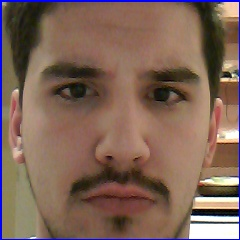
\includegraphics[width=.3\textwidth]{img/rui.jpg}\hfill

\includegraphics[width=.3\textwidth]{img/vadson.jpg}\hfill
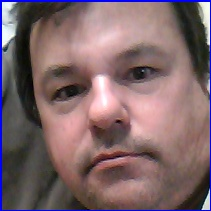
\includegraphics[width=.3\textwidth]{img/pedro.jpg}

\caption{Me, Roommate and Father}
\label{fig:figure3}

\end{figure}

When I compare these photos the values I had were the following:

\begin{figure}[!h]
	\center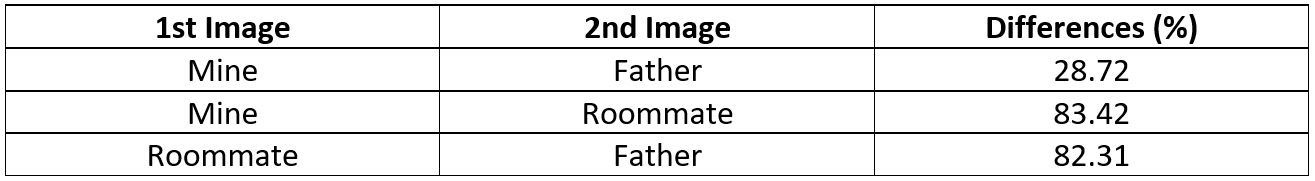
\includegraphics[width=1\textwidth]{img/Table.jpg}
	\caption{Tablue of Difference Values}
\end{figure}

\section{Conclusion}

In conclusion the project was well done and interesting results were achieved. We found an interesting way with some credability to compare two faces. It was also verty interesting to make this project because I never used OpenCV and Python in a project and it was a great experience to learn this two powerful tools.

\end{document}